%% This file was auto-generated by IPython.
%% Conversion from the original notebook file:
%% spline2.ipynb
%%
\documentclass[11pt,english,fleqn]{article}

%% This is the automatic preamble used by IPython.  Note that it does *not*
%% include a documentclass declaration, that is added at runtime to the overall
%% document.

\usepackage{amsmath}
\usepackage{amssymb}
\usepackage{graphicx}
\usepackage{ucs}
\usepackage[utf8x]{inputenc}

% needed for markdown enumerations to work
\usepackage{enumerate}

% Slightly bigger margins than the latex defaults
\usepackage{geometry}
\geometry{verbose,tmargin=3cm,bmargin=3cm,lmargin=2.5cm,rmargin=2.5cm}

% Define a few colors for use in code, links and cell shading
\usepackage{color}
\definecolor{orange}{cmyk}{0,0.4,0.8,0.2}
\definecolor{darkorange}{rgb}{.71,0.21,0.01}
\definecolor{darkgreen}{rgb}{.12,.54,.11}
\definecolor{myteal}{rgb}{.26, .44, .56}
\definecolor{gray}{gray}{0.45}
\definecolor{lightgray}{gray}{.95}
\definecolor{mediumgray}{gray}{.8}
\definecolor{inputbackground}{rgb}{.95, .95, .85}
\definecolor{outputbackground}{rgb}{.95, .95, .95}
\definecolor{traceback}{rgb}{1, .95, .95}

% Framed environments for code cells (inputs, outputs, errors, ...).  The
% various uses of \unskip (or not) at the end were fine-tuned by hand, so don't
% randomly change them unless you're sure of the effect it will have.
\usepackage{framed}

% remove extraneous vertical space in boxes
\setlength\fboxsep{0pt}

% codecell is the whole input+output set of blocks that a Code cell can
% generate.

% TODO: unfortunately, it seems that using a framed codecell environment breaks
% the ability of the frames inside of it to be broken across pages.  This
% causes at least the problem of having lots of empty space at the bottom of
% pages as new frames are moved to the next page, and if a single frame is too
% long to fit on a page, will completely stop latex from compiling the
% document.  So unless we figure out a solution to this, we'll have to instead
% leave the codecell env. as empty.  I'm keeping the original codecell
% definition here (a thin vertical bar) for reference, in case we find a
% solution to the page break issue.

%% \newenvironment{codecell}{%
%%     \def\FrameCommand{\color{mediumgray} \vrule width 1pt \hspace{5pt}}%
%%    \MakeFramed{\vspace{-0.5em}}}
%%  {\unskip\endMakeFramed}

% For now, make this a no-op...
\newenvironment{codecell}{}

 \newenvironment{codeinput}{%
   \def\FrameCommand{\colorbox{inputbackground}}%
   \MakeFramed{\advance\hsize-\width \FrameRestore}}
 {\unskip\endMakeFramed}

\newenvironment{codeoutput}{%
   \def\FrameCommand{\colorbox{outputbackground}}%
   \vspace{-1.4em}
   \MakeFramed{\advance\hsize-\width \FrameRestore}}
 {\unskip\medskip\endMakeFramed}

\newenvironment{traceback}{%
   \def\FrameCommand{\colorbox{traceback}}%
   \MakeFramed{\advance\hsize-\width \FrameRestore}}
 {\endMakeFramed}

% Use and configure listings package for nicely formatted code
\usepackage{listingsutf8}
\lstset{
  language=python,
  inputencoding=utf8x,
  extendedchars=\true,
  aboveskip=\smallskipamount,
  belowskip=\smallskipamount,
  xleftmargin=2mm,
  breaklines=true,
  basicstyle=\small \ttfamily,
  showstringspaces=false,
  keywordstyle=\color{blue}\bfseries,
  commentstyle=\color{myteal},
  stringstyle=\color{darkgreen},
  identifierstyle=\color{darkorange},
  columns=fullflexible,  % tighter character kerning, like verb
}

% The hyperref package gives us a pdf with properly built
% internal navigation ('pdf bookmarks' for the table of contents,
% internal cross-reference links, web links for URLs, etc.)
\usepackage{hyperref}
\hypersetup{
  breaklinks=true,  % so long urls are correctly broken across lines
  colorlinks=true,
  urlcolor=blue,
  linkcolor=darkorange,
  citecolor=darkgreen,
  }

% hardcode size of all verbatim environments to be a bit smaller
\makeatletter 
\g@addto@macro\@verbatim\small\topsep=0.5em\partopsep=0pt
\makeatother 

% Prevent overflowing lines due to urls and other hard-to-break entities.
\sloppy

\setlength{\mathindent}{0pt}
\setlength{\parindent}{0pt}
\setlength{\parskip}{8pt}
\begin{document}

Spline Egrileri Diyelim ki elimizde 4 $x_i,y_i$ noktasi var, ve bu
noktalardan gecen, hepsinden \emph{kesinlikle} gecen, yaklasiksal bir
egri olusturmak istiyoruz. Spline yontemi her iki nokta arasini farkli
bir kupsel (ucuncu derece) polinom ile temsil etmektir. Tekrar dikkat:
tum noktalari temsile edebilecek farkli polinomlari toplamiyoruz, her
aralikta baska bir polinom fonksiyonu parcasini devreye sokuyoruz.
Parcalar niye kupsel olarak secildi? Cunku kupsel bir egri yeterince
kavis saglayabilir ve ayni zamanda cok fazla inisli cikisli, sivri
degildir, yeterince puruzsuz bir egrinin ortaya cikmasini saglar.

\begin{codecell}
\begin{codeinput}
\begin{lstlisting}
im=imread("spline1.png"); imshow(im)
\end{lstlisting}
\end{codeinput}
\begin{codeoutput}
\begin{verbatim}
<matplotlib.image.AxesImage at 0xa0a89ac>
\end{verbatim}
\begin{center}
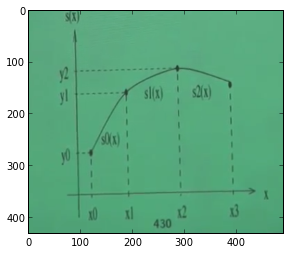
\includegraphics[width=0.7\textwidth]{spline2_files/spline2_fig_00.png}
\par
\end{center}
\end{codeoutput}
\end{codecell}
Her $i=0,..,n+1$ icin
\[ p(x) = p_i(x) = a_i + b_i(x-x_i) + c_i(x-x_i)^2 + d_i(x-x_i)^3
\ \ \ \label{1}
\]
kullanalim. Noktalar $x_i$ olarak gosteriliyor, ve her noktada aktif
olan bir $p_i$ spline olacak, o noktadan bir sonrakine kadar egriyi bu
$p_i$ tanimlayacak. Noktalarin sayisini $n$ yerine $n+1$ olarak aldik
boylece $n$ egri parcasi ile calismamiz mumkun olacak. Her spline bir
kubik polinom ise niye bu kubik polinomu en basit sekliyle
\[ p(x) = a_i + b_ix + c_ix^2 + d_ix^3 \]
olarak tanimlamadik? Cunku iki ustteki form ile calismak daha rahat.
Mesela, eger $x$ icin $x_i$ degrini verirsek, ki bu $x_1$ ya da $x_2$
olabilirdi, o zaman parantez icinde $x_i - x_i$ sayesinde tum terimler
sifir oluyor, geriye sadece $a_i$ kaliyor.

Parcalarin uclarinin birbirini tutmasi, ve tum seklin surekli, akiskan
bir sekilde gozukmesi icin ise birkac kosulu bizim tanimlamamiz, ve
zorlamamiz gerekli. Once en basit olani: bir onceki parca ile bir
sonraki parca orta nokta uzerinde ayni degere sahip olmali. $i=1,..,n+1$
icin
\[ p_i (x_{i+1}) = p_{i+1}(x_{i+1}) \]
Bir diger basit gereklilik, her $x_i$'ye tekabul eden spline fonksiyonun
elimizdeki $y_i$ degerini vermesi,
\[ p_i(x_i) = y_i \]
``Tum noktalardan kesinlikle gecmeli'' demistik. Son parca bir istisna
olusturuyor, bu son parcanin fonksiyonu hem son noktayi, hem de ondan
bir onceki nokta icin kullanilmali, bir onceden en sona kadar ayni
fonksiyon uzerindeyiz.
\[ p_{n}(x_n) = y_{n+1} \]
Sistemi daha detayli olarak gormek gerekirse, tum denklemleri yazalim,
\[ p_1(x)  = a_1 + b_1(x-x_1) + c_1(x-x_1)^2 + d_1(x-x_1)^3\]\[ p_2(x)  = a_2 + b_2(x-x_2) + c_2(x-x_2)^2 + d_1(x-x_2)^3\]\[ \vdots \]\[ p_n(x)  = a_n + b_n(x-x_n) + c_n(x-x_n)^2 + d_3(x-x_n)^3\]
Uc noktali soyle bir grafik dusunelim,

\begin{codecell}
\begin{codeinput}
\begin{lstlisting}
im=imread("spline2.png"); imshow(im)
\end{lstlisting}
\end{codeinput}
\begin{codeoutput}
\begin{verbatim}
<matplotlib.image.AxesImage at 0x95cdb2c>
\end{verbatim}
\begin{center}
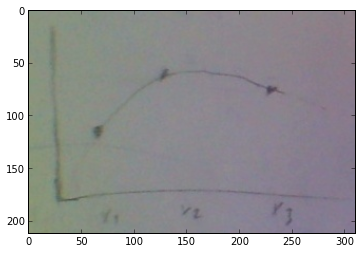
\includegraphics[width=0.7\textwidth]{spline2_files/spline2_fig_01.png}
\par
\end{center}
\end{codeoutput}
\end{codecell}
Ustte bahsettigimiz gibi, $p_1(x_1) = a_1 = y_1$ olacak, ve tum indisler
icin bu gecerli. Ayrica $x_2$ noktasinda bir onceki parca ve sonraki
parca ayni degere sahip olmali demistik, yani mesela $p_1$'in sonunda
(ustteki ilk parca) $x_2$ noktasi vardir, ve ayni noktada $p_2$
baslayacaktir, o noktada\[ p_1(x_2) = a_1 + b_1h_1 + c_1h_1^2 + d_1h_1^3  \]
ve bu denklem $p_2(x_2) = a_2 = y_2$'ye esit. Bir de, daha once gorduk,
$a_1 = y_1$ ise, o zaman
\[ y_2 = p_1(x_2) = y_1 + b_1h_1 + c_1h_1^2 + d_1h_1^3 \]
haline gelir. Hepsini birarada yaziyoruz ($y$'yi sag tarafa aldik)
\[ y_1 + b_1h_1 + c_1h_1^2 + d_1h_1^3 = y_2 \ \ \ \label{2} \]\[ y_2 + b_2h_2 + c_2h_2^2 + d_2h_2^3 = y_3 \]\[ \vdots \]\[ y_n + b_nh_n + c_nh_n^2 + d_nh_n^3 = y_n \]
ki $h_1 \equiv x_2 - x_1$, $h_2 \equiv x_3 - x_2$ olarak tanimladik,
$\equiv$ isareti ``tanimlamak (defined as)'' anlamina geliyor, $h$ harfi
bir tur kisaltma olarak kullanildi. Fakat kesintisizlik icin parcalarin
uclarinin bitismesi yeterli degil. Mesela alttaki figurun de uclari
birlesiktir,

\begin{codecell}
\begin{codeinput}
\begin{lstlisting}
im=imread("spline3.png"); imshow(im)
\end{lstlisting}
\end{codeinput}
\begin{codeoutput}
\begin{verbatim}
<matplotlib.image.AxesImage at 0x980e68c>
\end{verbatim}
\begin{center}
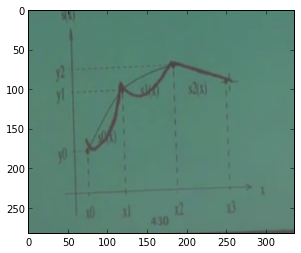
\includegraphics[width=0.7\textwidth]{spline2_files/spline2_fig_02.png}
\par
\end{center}
\end{codeoutput}
\end{codecell}
Demek ki ek bazi sartlar lazim. Bu ek sart ``sureklilik'' olabilir.
Mesela alttaki ornek surekli degildir.

\begin{codecell}
\begin{codeinput}
\begin{lstlisting}
im=imread("spline5.png"); imshow(im)
\end{lstlisting}
\end{codeinput}
\end{codecell}
Ya da daha iyisi, fonksiyonun her noktada ``turevi alinabilir'' olma
sarti. Mesela altta koyu yuvarlakli gosterilen noktada fonksiyonun
turevi alinamaz.

\begin{codecell}
\begin{codeinput}
\begin{lstlisting}
im=imread("spline4.png"); imshow(im)
\end{lstlisting}
\end{codeinput}
\begin{codeoutput}
\begin{verbatim}
<matplotlib.image.AxesImage at 0xa05dd2c>
\end{verbatim}
\begin{center}
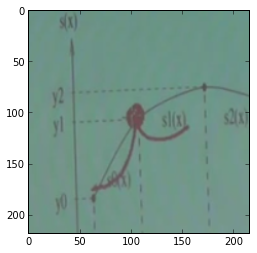
\includegraphics[width=0.7\textwidth]{spline2_files/spline2_fig_03.png}
\par
\end{center}
\end{codeoutput}
\end{codecell}
O zaman sarti koyalim -- Fonksiyonun her noktasinda, ikinci turev
surekli alinabilmeli. Bu cok agir / net bir sart aslinda, ve hakikaten
cok puruzsuz (smooth) fonksiyonlara sebebiyet veriyor. Simdi bunun ne
anlamina biraz daha yakindan bakalim. Bilirsiniz futbol sahalarinin
etrafinda kosu alani vardir. Bu alan soyledir.

\begin{codecell}
\begin{codeinput}
\begin{lstlisting}
im=imread("spline6.png"); imshow(im)
\end{lstlisting}
\end{codeinput}
\begin{codeoutput}
\begin{verbatim}
<matplotlib.image.AxesImage at 0x9c7ebcc>
\end{verbatim}
\begin{center}
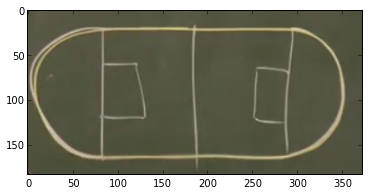
\includegraphics[width=0.7\textwidth]{spline2_files/spline2_fig_04.png}
\par
\end{center}
\end{codeoutput}
\end{codecell}
Bu sekil iki ayri figurun birlesimidir aslinda, duz cizgiler ve iki tane
yari cember. Ustteki duz cizgili kisim sonsuz kere turevi alinabilir bir
fonksiyondur. Degil mi? Duz cizgi sabit bir sayidir, 1. turev sifir,
ikinci turev yine sifir, boyle gider. Peki yari cember olan kisimlar?
Ayni sekilde. Peki her noktada durum boyle midir? Kritik noktalar ufak
yuvarlaklarla gosterilen yerler (altta)

\begin{codecell}
\begin{codeinput}
\begin{lstlisting}
im=imread("spline7.png"); imshow(im)
\end{lstlisting}
\end{codeinput}
\begin{codeoutput}
\begin{verbatim}
<matplotlib.image.AxesImage at 0x9b3070c>
\end{verbatim}
\begin{center}
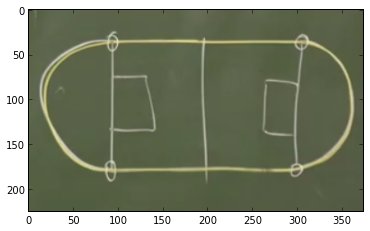
\includegraphics[width=0.7\textwidth]{spline2_files/spline2_fig_05.png}
\par
\end{center}
\end{codeoutput}
\end{codecell}
Bu noktalarda kac kere ``surekli turevler'' alinabilir? Cevap, sadece
bir kere. Cunku iki kere turev alininca ne olacagina bakalim, duz
kisimda ikinci, ucuncu, vs.~turev sifir. Peki yari cember? Onun ikinci
turevi sifir olmayan sabit bir sayi. O zaman fonksiyonun tamaminin (duz
cizgi ve yari cemberin beraber) 2. turevini grafiklesek, soyle bir sekil
ortaya cikardi,

\begin{codecell}
\begin{codeinput}
\begin{lstlisting}
im=imread("spline8.png"); imshow(im)
\end{lstlisting}
\end{codeinput}
\begin{codeoutput}
\begin{verbatim}
<matplotlib.image.AxesImage at 0x9aadd0c>
\end{verbatim}
\begin{center}
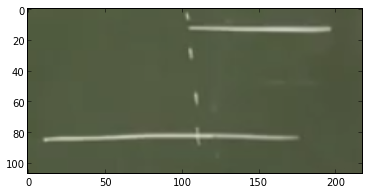
\includegraphics[width=0.7\textwidth]{spline2_files/spline2_fig_06.png}
\par
\end{center}
\end{codeoutput}
\end{codecell}
ve bu grafikte goruyoruz ki bir ziplama var. Bu ziplama yuzunden
sureklilik (2. turevde) bozulmus oldu. O zaman spline duzgun, puruzsuz
olsun istiyorsak, her noktada, yani baglanti noktalarinda, sagdaki ve
soldaki parcanin birinci ve ikinci turevinin ayni olmasi sartini
koyabiliriz, o zaman bu noktalarda fonksiyonun tamami iki kere surekli
turevi alinabilir hale gelir. Parcalarin kendisi uzerinde bu sarti
tanimlamaya gerek yok, cunku orada polinom kullanacagimizi belirttik
zaten, polinomlar sonsuz kere surekli turevi alinabilen objelerdir.

Denklem sistemimize iki tane daha sart gerekiyor. Bu sartlar fonksiyonun
ilk noktada ve son noktada ikinci turevinin sifir olmasi sarti olabilir.
Her hangi yondeki bir cizgi $y = ax + b$`nin iki kere turevi alininca
sifir gelir, yani bu sart fonksiyonumuzun son noktalarda, fonksiyonun
``asagi yukari ayni yonde'' olacak sekilde duz olarak devam etmesi
anlamina geliyor. Yaklasiksal baglamda fena bir sart degil.

O zaman ana formullerimize donelim, ve mesela $p_1(x),p_2(x)$'in
turevini alalim,
\[ p_1'(x) = b_1 + 2c_1h_1 + 3d_1h_1^2 \]\[ p_2'(x) = b_2 + 2c_2h_2 + 3d_2h_2^2 \]\[ \vdots \]
Turevleri esitleyelim $p_1'(x_2) = p_2'(x_2)$.
\[ p_1'(x_2) = b_1 + 2c_1h_1 + 3d_1h_1^2 \]\[  p_2'(x_2) = b_2 \]
Ustteki niye sadece $b_2$ oldu? Cunku $x_i-x_i$ numarasi onun icin de
gecerli, geriye sadece $b_2$ kaldi. Hepsi bir arada
\[  b_1 + 2c_1h_1 + 3d_1h_1^2  = b_2 \ \ \ \label{3}\]\[  b_2 + 2c_2h_2 + 3d_2h_2^2 = b_3 \]\[ \vdots \]\[  b_{n-1} + 2c_{n-1}h_{n-1} + 3d_{n-1}h_{n-1}^2 =  b_n \]
Ikinci turevler icin benzer bir durum var, bu sefer sol taraftan $b$'ler
yokoluyor,
\[ 2c_1 + 6d_1h_1 = 2c_2 \ \ \ \label{4} \]\[ 2c_2 + 6d_2h_2 = 2c_3 \]\[ \vdots \]\[ 2c_{n-1} + 6d_{n-1}h_{n-1} = 2c_n \]
Ilk ve son ikinci turevi sifira esitlemeyi unutmayalim. Son turev
\[ 2c_n + 6d_nh_n = 2c_{n+1} = 0 \]
Ilk turev \[ p_1''(x_1) =  c_1 + 6d_1(x_1-x_1)  = c_1 = 0\]\[ 6d_1(x_1-x_1) \] sifir olur

Denklem (4)'den baslayan blogu tekrar duzenlersek,
\[ d_1 = \frac{ c_2 - c_1}{3h_1} \ \ \ \label{5} \]\[ d_2 = \frac{ c_3 - c_2}{3h_2} \]\[ \vdots \]\[ d_n = \frac{ c_{n+1} - c_n}{3h_n} \]
Ustteki denklemleri (2) ve (3)'e geri koyarsak,
\[ b_1 + \frac{ c_2 + 2c_1}{3}h_1 = s_1 \ \ \ \label{7} \]\[ b_2 + \frac{ c_3 + 2c_2}{3}h_1 = s_2 \]\[ \vdots \]\[ b_n + \frac{ c_{n+1} + 2c_n}{3}h_n = s_n \]
ki $s_1 \equiv \frac{y_2 - y_1}{h_1}, s_2 \equiv \frac{y_3 - y_2}{h_2}$.

\begin{enumerate}[(1)]
\setcounter{enumi}{2}
\item
  ifadesini alip tekrar duzenlersek,
\end{enumerate}\[  2c_1h_1 + 3d_1h_1^2  = b_2 - b_1\]
$3d_1h_1$ icin baska bir ifade kullanabiliriz, eger (5)'i tekrar
duzenlersek,
\[ 3h_1d_1 = c_2 - c_1\]
ve iki ustteki formule koyarsak
\[  2c_1h_1 + (c_2 - c_1)h_1  = b_2 - b_1\]\[  2c_1h_1 + c_2h_1 - c_1h_1  = b_2 - b_1\]\[  c_1h_1 + c_2h_1  = b_2 - b_1\]\[  (c_1 + c_2) h_1  = b_2 - b_1\]
Bu ifade tum $i$ noktalari icin gecerli, hepsi bir arada
\[  (c_1 + c_2) h_1  = b_2 - b_1 \ \ \ \label{6}\]\[  (c_2 + c_3) h_2  = b_3 - b_2\]\[ \vdots \]\[  (c_{n-1} + c_n) h_{n-1}  = b_n - b_{n-1}\]
(7)'deki ardi ardina gelen denklemleri birbirinden cikartip sonucu 3 ile
carparsak,
\[ c_1h_1 + 2c_2(h_1 + h_2) + c_3h_2 = 3(s_2 - s_1) \]\[ c_2h_2 + 2c_3(h_2 + h_3) + c_4h_3 = 3(s_3 - s_2) \]\[ \vdots \]\[ c_{n-1}h_{n-1} + 2c_n(h_{n-1} + h_{n}) + c_{n+1}h_n = 3(s_n - s_{n-1}) \]
Bu formuller birarada dusunulurse, bilinmeyenleri $c_2,c_3,..,c_n$ olan
normal (ordinary) $n-1$ tane lineer denklemdirler, ve bir matris carpimi
olarak dusunulebilirler.

$c_1h_1$ matris formunda yok cunku $c_1=0$.
\[ 
\left[\begin{array}{cccccc}
2(h_1+h_2) & h_2 & 0 & 0 & ... & 0 \\
h_2 & 2(h_2+h_3) & h_3 & 0 & .. & 0  \\
0 & h_3 & 2(h_3+h_4) & h_4 & .. & 0 \\
0 & 0 & h_4 & 2(h_4+h_5) & ... & 0 \\
\vdots & \vdots & \vdots & \vdots & \ddots & \vdots  \\
0 & 0 & .. & 0 & h_{n-1} & 2(h_{n-1}+h_n) 
\end{array}\right]
\left[\begin{array}{r}
c_2 \\ c_3 \\ \vdots \\ c_n
\end{array}\right]
 \]
Bu denklem sag tarafta suna esit
\[ 
\left[\begin{array}{r}
3(s_2 - s_1) \\
3(s_3 - s_2) \\
3(s_4 - s_3) \\
\vdots \\
3(s_n - s_{n-1}) 
\end{array}\right]
 \]
Bir ucgen kosegen (tridiagonal) matris iki tane ikili kosegen
(bidiagonal) matrisin carpimina esittir. LU carpanlarina ayirma islemi
de (bkz Lineer Cebir Ders 4) bize bu matrisleri saglayacaktir.
\[ Ax = b \]
su hale gelir
\[ LUx = b \]
Simdi eger $Ux = y$ kabul edersek, yani yeni bir degiskeni dahil
edersek, $L$'i bulduktan sonra
\[ Ly = b \]
kabul edebiliriz, ve bu formulu de $y$ icin cozmek cok kolaydir. Sonra
cozulen $y$'yi alip geriye sokma (backsubstitution) ile $x$'i buluruz,
yani
\[ Ux = y \]
denklemini cozeriz.

\begin{codecell}
\begin{codeinput}
\begin{lstlisting}
import scipy.linalg as lin

a = np.array( [[3.,-3.,0,0],
               [-3.,8.,-2.,0],
               [0,1.,2.,4.],
               [0,0,-2.,6.]])

p,l,u = lin.lu(a)

Ly = np.array([[7.,8.,2.,-3.]])

y = lin.solve(l,Ly.T)

x = lin.solve(u,y)
x
\end{lstlisting}
\end{codeinput}
\begin{codeoutput}
\begin{verbatim}
array([[ 5.44047619],
       [ 3.10714286],
       [ 0.26785714],
       [-0.41071429]])
\end{verbatim}
\end{codeoutput}
\end{codecell}
Spline yontemine donersek, elimizdeki veri ve kod soyle olsun

\begin{codecell}
\begin{codeinput}
\begin{lstlisting}
import scipy.linalg as lin

xx = np.array([4.,9.,12.,16.,22.])

yy = np.array([157.,41.,145.,92.,7.])

h = np.diff(xx)

dy = np.diff(yy)

s = dy / h

ds = np.diff(s)

s3 = 3 * ds

a = np.array([[ 2*(h[0]+h[1]), h[1], 0],
              [ h[1], 2*(h[1]+h[2]), h[2]],
              [ 0, h[2], 2*(h[2]+h[3])]])

p,l,u = lin.lu(a)

y = lin.solve(l,s3.T)

c = lin.solve(u,y)
c
\end{lstlisting}
\end{codeinput}
\begin{codeoutput}
\begin{verbatim}
array([ 13.45756677, -13.90702275,   2.64390455])
\end{verbatim}
\end{codeoutput}
\end{codecell}
$c$'ler bulunduktan sonra $h$'lerle beraber kullanilarak $d$'ler
bulunur, vs, ve tum spline parcalarinin katsayilari ortaya cikartilir.

Kaynaklar

http://spartan.ac.brocku.ca/\ensuremath{\sim}jvrbik/MATH2P20/notes.pdf

http://www.youtube.com/watch?v=3rHBCglD1LQ

http://www.youtube.com/watch?v=nA0YpqraP9A

\end{document}
